\section{Introduction}
This book is a high level view of technologies and their potential within the developing digital society narrative, focusing around the transmission of value within and across immersive global networks, with a further focus on the Bitcoin monetary network.\par
Cybersecurity is top of the list of concerns in the \href{https://digital-strategy.ec.europa.eu/en/policies}{EU digital society strategy}, just ahead of digital inclusion, so we started out with security best practices in mind, and we tried to end the investigation with inclusion. We aimed to support small and especially developing companies in our sector, giving them a foot in the door on a global stage, without their costs spiralling? \par
Fortunately, we discovered a wealth of carefully crafted open source tools which can support this. \href{https://opensource.org/osd}{Open source software} is software that is available with source code that can be modified and distributed by anyone. The model extended into other creative works through things like the \href{https://creativecommons.org/licenses/}{Creative Commons} licenses, which is itself an \href{https://open-stand.org/about-us/principles/}{`open standard'}. We will return to these themes throughout the book, and both this text and the supporting code are open source. This means that anyone can access, use, and modify the source code for their own purposes. Open source software is often developed and maintained by a community of volunteers, and it can be freely distributed and modified. This approach to software development allows for more collaboration and innovation, as well as greater transparency and security. Many popular software programs, such as the Linux operating system and the Apache web server, are open source.\par
We have tried to assemble the tools we found, cogently, to deliver an open source kit for experimentation, to curious technically individuals and groups, and we have applied our own security knowledge on top of an already top class set of tools. It’s certainly not production ready, but it's good enough to commit small amounts of money into, and collaboration with Pathway is welcomed.\par
Whilst researching, it seemed that every door we opened was full of interesting and useful treats. What was supposed to be a short technical paper quickly became a 200-page book, and a deployable virtual machine stack, with a dozen different open source components in it. \par
This book supports the software stack, which supports anyone who thinks this material might be useful. Below is a précis of the chapters of the book, which will hopefully give an insight into what ``this stuff'' is. The reader can decide to download the book and the system ``How To'' guide. All of it is open source, all of it can be contributed to on GitHub, all of it will be developed forward, and none of it is really finished yet.\par
Chapter 1 starts with an introduction to the book which is about value transmission, with distributed trust, in global digital society and mixed reality systems. \par
Next is a summary of Web3, as it stands right now. Web3 is a complex term that is cropping up far more in the technical press, so we wanted explain what it might mean. Honestly, it’s still pretty confusing. There are a bunch of legacy explanations which are Web3.0 (note the `0' there), but these are withering on the vine. Then there’s the new VC funded, super hyped, and potentially useless Web3 incarnations, which again cover a slew of intersecting technologies. Note they dropped the zero to reboot the brand! This doesn’t mean there’s nothing to see here. The astonishing amount of \href{https://mirror.xyz/tr3butor.eth/AlZPMq_syymAoi8M1VVb2xES9Twj1OeetJbEE7EWhiw}{money and developer talent}, and the clear market hunger for things like NFTs (non-fungible tokens) suggest that there’s a future for Web3, it’s just really unclear if this is inherently valuable or just hype.\par
In the next chapter we took a look at blockchain, which is very intersectional with Web3. Even on its own this is a complex emergent set of disciplines. \par
The blockchain chapter was especially interesting to research. It turns out there’s a \textit{lot} of ways to get this technology wrong. Even very appealing options on paper, turn out to have very shaky foundations. There are valuable things here, but given the complexity and scope, we decided to focus on the most promising of the technology stacks; the Bitcoin network.\par
Even Bitcoin isn’t just Bitcoin any more. It’s a swarm of open source tools which can (in theory) accomplish a great many things. These are illustrated well in Figure \ref{fig:ecosystemmap}. 
\begin{figure*}[ht]\centering % Using 
	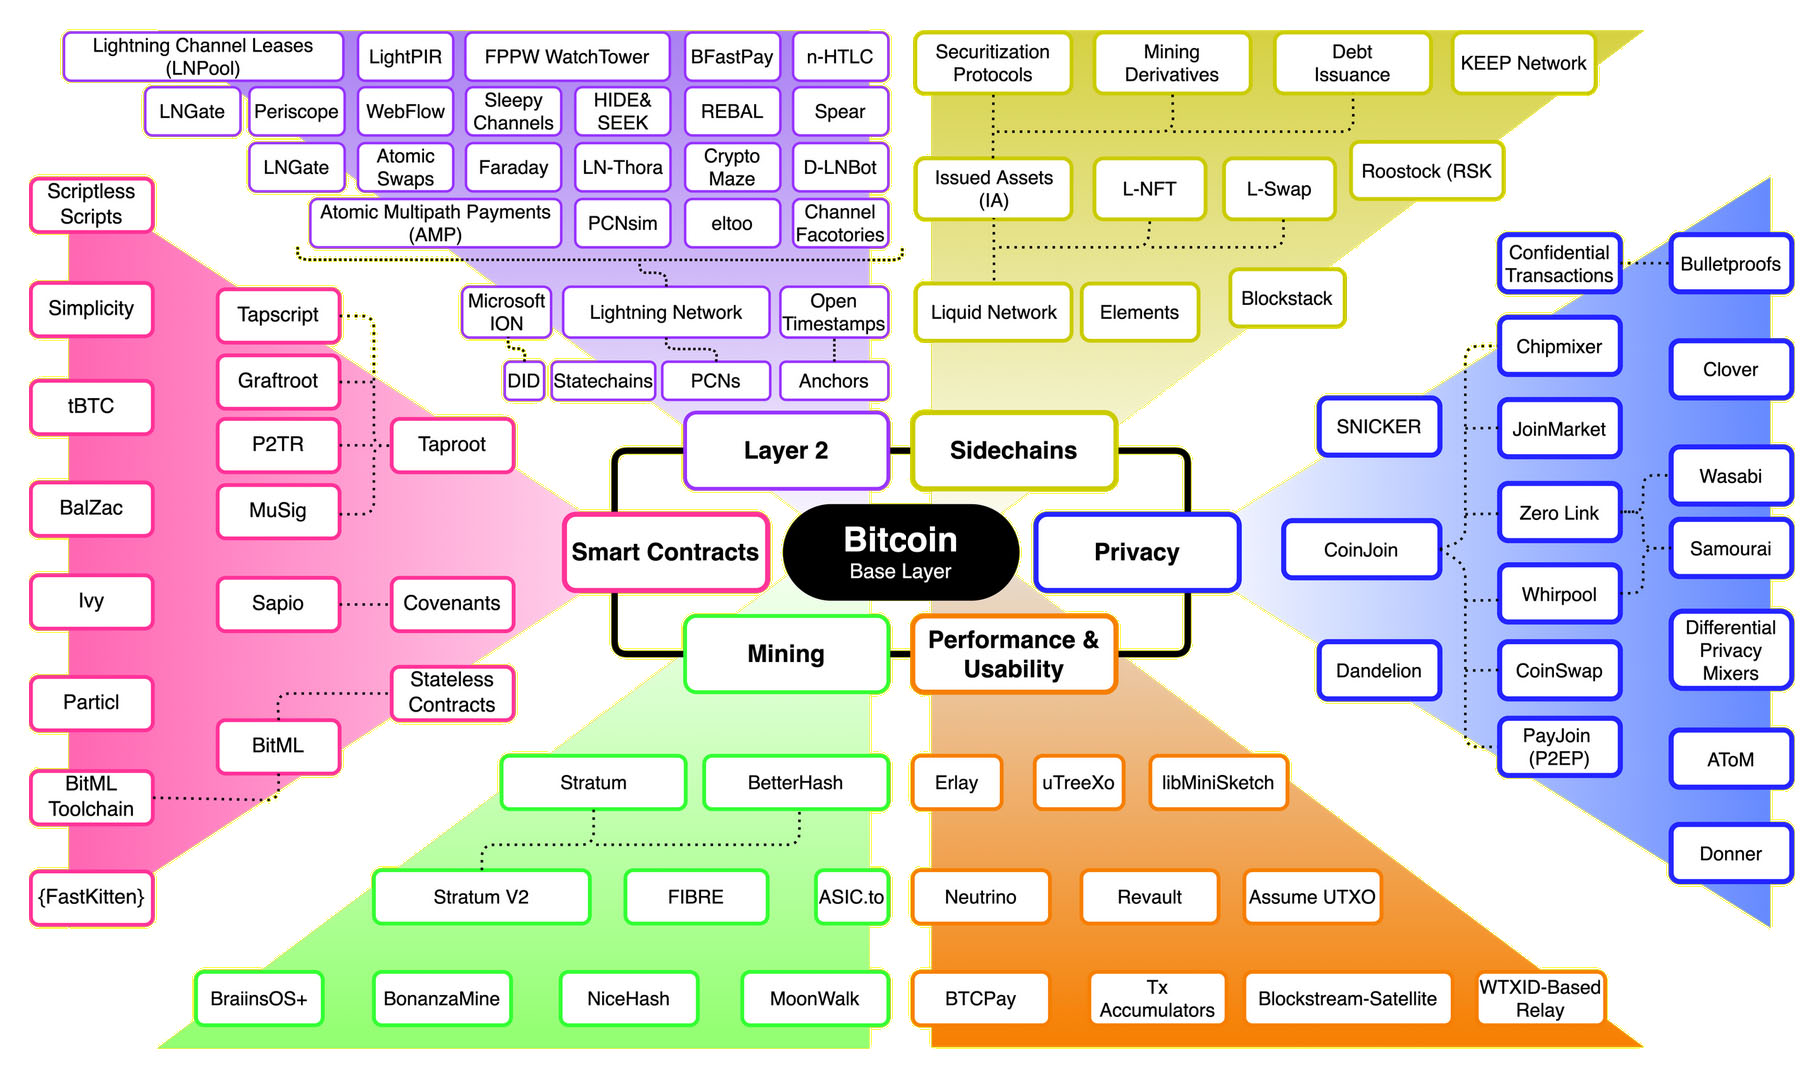
\includegraphics[width=\linewidth]{ecosystemmap}
	\caption{The Open Source Map of The Bitcoin Protocol Ecosystem \href{https://www.ekosys.org/}{maintained by Lucas Nuzzi} of Coinmetrics}
	\label{fig:ecosystemmap}
\end{figure*}
These newer, ancillary elements to Bitcoin, are emergent right now. Some of them won’t be around until next year, and it’s questionable whether they will even work out. With that said we aren't convinced by the value proposition of of Ethereum, and there’s enough Bitcoin tooling for us to cherry pick useful components. We map those forward into our metaverse product.\par
%It seems possible that the features which are important to Web3, can also (potentially) arise from the Bitcoin technology that we think most secure. This was somewhat unexpected, so we started mapping that over too.\par
The next chapter is about Money. In expanding our research on Bitcoin, we found that it’s impossible to think about the tech without opening up a whole line of questions about money itself. This is fine because we set out to look at global value transfer for business. It’s not a trivial subject though, and this section tries to overview why value and Bitcoin are so enmeshed, then what other options there might be in the end (because Bitcoin has kicked off a whole slew of global adoption outside of itself).\par
The distributed identity management, and trust chapter follows. Identity management is important for digital society and potentially crucial to metaverse applications which have a value transaction layer. It’s not an easy section to write about, because there’s a lot of research, it’s not our field, and finding the value to SMEs has actually been very difficult. It's by no means clear that blockchain is the right tool for this component, and newer cryptographic products are emerging.\par %This section is likely to be overhauled a few times in the coming months as we settle on technologies that we believe are simple and secure enough.\par
In chapter 7 we take another look at NFTs. It’s impossible to ignore this stuff now. It’s fundamentally a bit broken, but there are probably use cases, and the money and development attention it’s getting are incredible. We try to navigate our hypothetical virtual production partners through this as best we can. \par %It’s not that we didn’t understand it completely, just that the tech moves so very fast that it’s impossible to even describe what’s going on accurately at any given point. \par
We’re actually pretty excited about future versions of `digital assets', based around Bitcoin, because that allows us to keep just one software stack, minimising the threat surface. We’ve mapped that forward into the open source tools that we recommend.\par
Chapter 8 is a big one for us as it’s our research area prior to opening up the Bitcoin box(es). Metaverse, or at least one of the current definitions of metaverse, is just social interaction in mixed reality (VR/AR/XR). We’ve been studying that for decades, so this section is more academic and tried to boil down what we think is most important. The choices we made here guided us toward the selection of free and open source metaverse software.\par
We also take a look at the other definitions of `metaverse' which are doing the rounds on the web, try to unpick which is which, and what they are for, and attempt to weave back together the best of both. This ends up looking a bit like the Venn in Figure \ref{fig:landscapevenn}, where we have transmission of provable identity, non-fungible tokens bearing value or data, distributed files, actual money (including micropayments) and a social layer based on our best knowledge about mixed reality. In the end we abandon the word metaverse and settle on `digital society' as our preferred term.\par
It's exceptionally fortunate timing for this book that the UK government has signalled enthusiasm for so called `stablecoins' at the same time that the Bitcoin network is being upgraded to transmit these GBP equivalent tokens around. This gives us a very good idea what it is we can build into our application stack.\par 
Past this stage in the book we get into the murky and half developed tail end, where we’re interfacing with our design choices, and the stack which can be deployed into the cloud.\par

\begin{figure*}[ht]\centering % Using 
	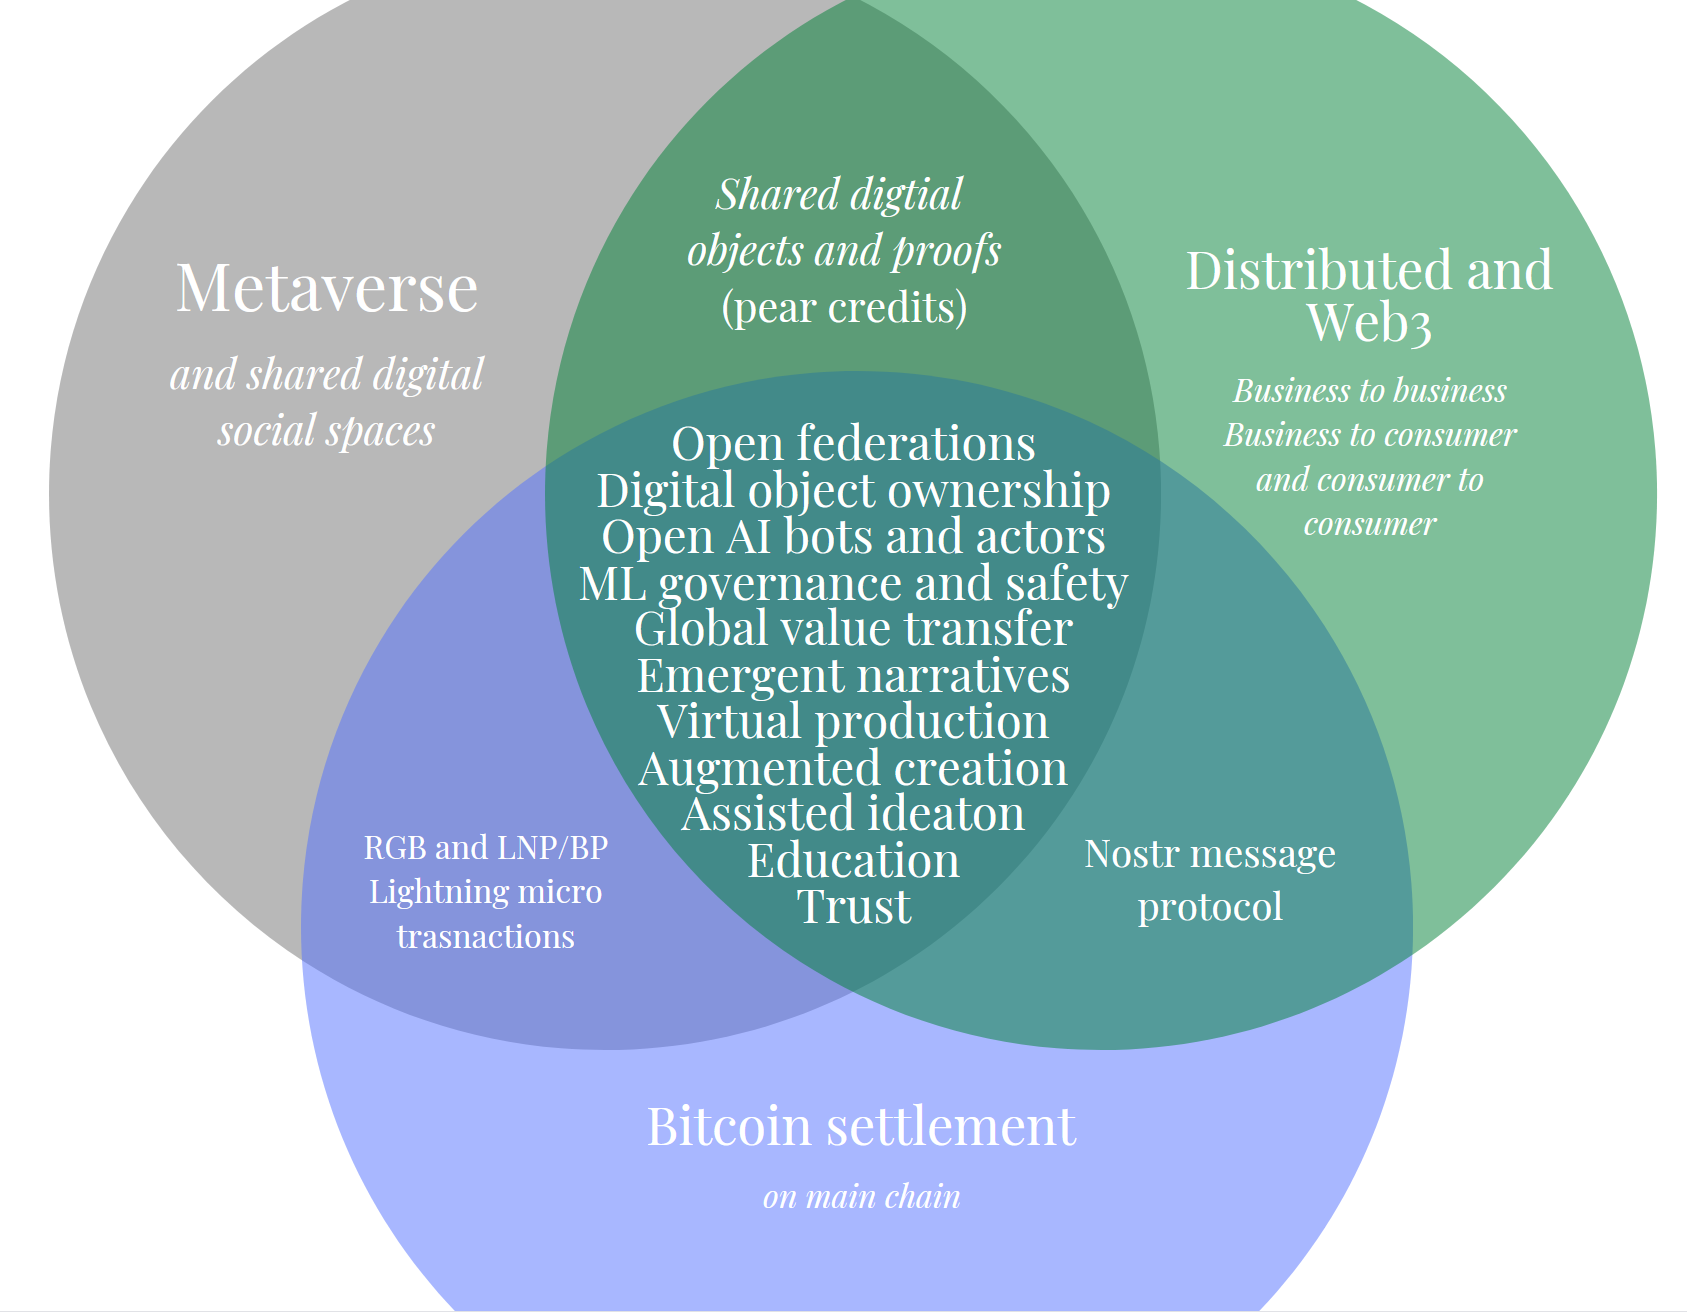
\includegraphics[width=\linewidth]{landscapevenn}
	\caption{Web 3, Metaverse, and Bitcoin are intersectional technologies.}
	\label{fig:landscapevenn}
\end{figure*}

As adoption of these technologies increases it will be necessary for people, and AI actors, to pass economic value between themselves. These `goods and services' interactions, within the digital and virtual social spaces should be underpinned by a trust system, which scales globally and presents low friction. Current secure international payment rails are poorly suited to such interactions; indeed it is likely with legacy systems, that parties would be forced to leave the metaverse application, and instead navigate their banking applications to exchange value with overseas entities in a secure fashion. This might conceivably take several days.\par 
Fortunately, the whole landscape of money and \href{https://www.omfif.org/futureofpayments2021/}{value transfer is changing}. Huge global financial players are entering the space. HSBC have \href{https://sandboxgame.medium.com/hsbc-to-become-the-first-global-financial-services-provider-to-enter-the-sandbox-c066e4f48163}{just bought} metaverse `land' in The Sandbox, JP Morgan have \href{https://www.forbes.com/sites/ronshevlin/2022/02/16/jpmorgan-opens-a-bank-branch-in-the-metaverse-but-its-not-for-what-you-think-its-for/?sh=2fbd1e90158d}{opened a `lounge'} in another. The worlds largest hedge fund Bridgewater is stepping into \href{https://uk.finance.yahoo.com/news/bitcoin-latest-price-crypto-ray-dalio-bridgewater-investment-fund-ethereum-094946686.html}{acquisition of digital assets}, and the world's largest pension fund manager Blackrock \href{https://blog.coinbase.com/coinbase-selected-by-blackrock-provide-aladdin-clients-access-to-crypto-trading-and-custody-via-b9e7144f313d}{partnered with crypto behemoth Coinbase} and is adding these asset to their management engine (which manages tens of trillions of dollars). America's oldest bank \href{https://www.bnymellon.com/emea/en/about-us/newsroom/press-release/bny-mellon-launches-new-digital-asset-custody-platform-130305.html}{BNY Mellon}, and even the Nasdaq stock exchange are \href{https://www.nasdaq.com/articles/nasdaq-to-launch-institutional-bitcoin-crypto-custody-services\%3A-report}{offering service to institutional clients}, and Fidelity asset management are about to add \href{https://www.wsj.com/articles/fidelity-weighs-bitcoin-trading-on-brokerage-platform-11663008698}{Bitcoin to their pension plans}. Fidelity are also offering a \href{}{dedicated metaverse tradable fund}, and considering more direct product offerings through their retail investment engine. \href{https://www.citivelocity.com/citigps/metaverse-and-money/}{Citigroup have a minisite} dedicated to ``Metaverse and Money''. The front page of Goldman Sachs recently says it all (Figure \ref{fig:goldmanFront}).\par
\begin{figure}[ht]\centering % Using \begin{figure*} makes the figure take up the entire width of the page
	\includegraphics[width=0.5\linewidth]{goldmanFront}
	\caption{The landing page of global\\financial giant Goldman Sachs shows the hype.}
	\label{fig:goldmanFront}
\end{figure}
In Gartners \href{https://www.itp.net/emergent-tech/gartner-says-nfts-metaverse-web3-will-expand-immersive-experiences}{2022 hype cycle report} one of their three ``trend themes'' says: \textit{``The future of digital experience is immersive. A collection of emerging technologies supports such experiences through dynamic virtual representations, environments and ecosystems of customers and people, as well as new modes of user engagement. With these technologies, individuals can control their own identities and data and experience virtual ecosystems that can be integrated with digital currencies. These technologies help reach customers in new ways to strengthen or open new revenue streams.
The technologies to watch that deliver evolving and expanding immersive experiences are metaverse, non-fungible tokens (NFTs), super apps and Web3, decentralized identity, digital humans, digital twin of the customer and internal talent marketplaces.''}\par
Of their recent investments KPMG global said: \textit{``We've invested in a strong cryptoassets practice and we will continue to enhance and build on our capabilities across Decentralized Finance (DeFi), Non-Fungible Tokens (NFTs) and the Metaverse, to name a few''}. This is not to say that all fund managers are so positive. PGIM who manage over a trillion pounds globally have come out very strongly against the technology, with a \href{https://www.pgim.com/megatrends/cryptocurrency-investing/bitcoin?}{slew of reports} to warn off investors (Figure \ref{fig:pgim}).\par
\begin{figure}[ht]\centering 	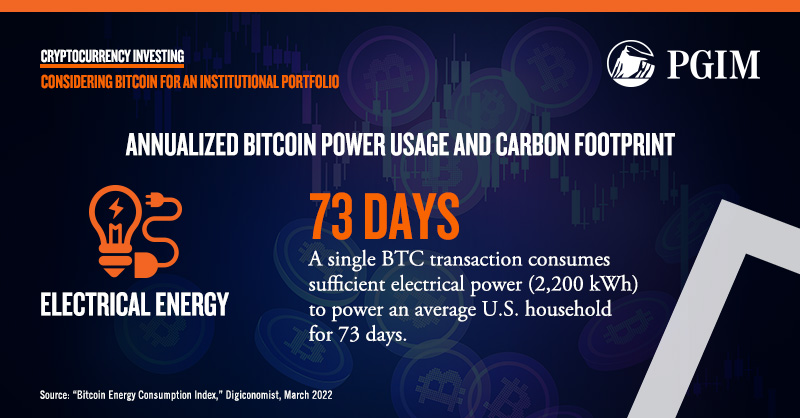
\includegraphics[width=0.5\linewidth]{pgim}
	\caption{PGIM cite `digiconomist', a prominent critic.}
	\label{fig:pgim}
\end{figure}
It's possible that for such huge organisations it makes better business sense to take a punt on hype bubbles like this, than to do a proper due diligence with a team of internal staff who understand their business. These endorsements should be taken with a large pinch of salt. As \href{https://newsletter.fintechtakes.com/p/metaverse-branches?s=r}{Alex Johnson says}: \textit{``At some point in the future, it’s possible that the digital worlds being built today will have aggregated sufficient user attention and engagement that financial services companies will need to invest in the metaverse as an acquisition and customer service channel. But we’re not there yet. Until the metaverse is a little less empty, resist the temptation to colonize it with branches and billboards.''}\par
Meanwhile, Meta (ex Facebook) are launching their own \href{https://archive.ph/coyp2}{META Web3 and metaverse} token (after abandoning Libre, their global cryptocurrency), and \href{https://www.coinbase.com/blog/announcing-coinbase-google-cloud}{Google have formed a strategic partnership} with Coinbase, and \href{https://blog.youtube/inside-youtube/innovations-for-2022-at-youtube/}{recently blogged}: \textit{``Web3 also opens up new opportunities for creators. We believe new technologies like blockchain and NFTs can allow creators to build deeper relationships with their fans. Together, they'll be able to collaborate on new projects and make money in ways not previously possible. For example, giving a verifiable way for fans to own unique videos, photos, art, and even experiences from their favourite creators could be a compelling prospect for creators and their audiences. There's a lot to consider in making sure we approach these new technologies responsibly, but we think there's incredible potential as well. Finally, we couldn't have a piece about innovation without touching on the metaverse! We're thinking big about how to make viewing more immersive. ''}\par
It's already the case that the recent bubble of \href{https://www.forbes.com/sites/paultassi/2022/03/10/interest-in-nfts-and-the-metaverse-is-falling-fast/?}{hype is dwindling}, but the enormous investment into teams and startups will potentially bear fruit in the next couple of years, and this perhaps has implications for small and medium-sized enterprises. PathwayXR is both an SME and well positioned in this highly convergent moment.\par
In the UK the government has stated it's ambition to be a \href{https://www.gov.uk/government/news/government-sets-out-plan-to-make-uk-a-global-cryptoasset-technology-hub}{global cryptoasset technology hub}, and announced plans for the Royal Mint to issue a (novelty) NFT. Fuller, Economic Secretary to the Treasury \href{https://drive.google.com/file/d/19ZYKLeT-ds3TueTpqSM22MUqB4gmN_Pl/view}{said in a speech}: \textit{``We want to become the country of choice for those looking to create, innovate and build in the crypto space [...] By making this country a hospitable place for crypto technologies, we can attract investment, generate new jobs, benefit from tax revenues, create a wave of ground breaking new products and services, and bridge the current position of UK financial services into a new era.''}\par
Like the assertion by major global businesses it is too early to tell how `sticky' these claims are. Indeed the findings of a recent treasury committee looking at the sector suggest that there is much work to do, with \href{https://committees.parliament.uk/committee/158/treasury-committee/news/175634/treasury-committee-85-of-crypto-firms-failed-to-meet-minimum-standards-according-to-fca/}{85\% of companies} failing to comply with \textit{existing} law. The UK legal system is clear in it's view that all crypto assets \href{https://blockchain.bakermckenzie.com/2020/02/03/uk-court-confirms-bitcoins-status-as-property/}{are `property'}.\par
A Law Commission consultation on ``digital assets'' \href{https://s3-eu-west-2.amazonaws.com/lawcom-prod-storage-11jsxou24uy7q/uploads/2022/07/Digital-Assets-Summary-Paper-Law-Commission-1.pdf}{has proposed a new \textbf{third category} of property}:
\textit{\begin{itemize}
\item it is composed of data represented in an electronic medium, including in the
form of computer code, electronic, digital or analogue signals;
\item it exists independently of persons and exists independently of the legal system;
\item it is rivalrous such that use by one  prejudices the ability of others;
\end{itemize}
}
Consensus seems to be that this is a thorough paper, and demonstrates strong knowledge of digital assets by the authors. \par
Gartner's \href{https://en.wikipedia.org/wiki/Gartner_hype_cycle}{hype cycle} 2022 features \href{https://www.gartner.com/en/articles/what-s-new-in-the-2022-gartner-hype-cycle-for-emerging-technologies}{Web3, distributed identity, NFTs, and Metaverse} and can be seen in Figure \ref{fig:gartners}.\par
\begin{figure}[ht]\centering % Using 
	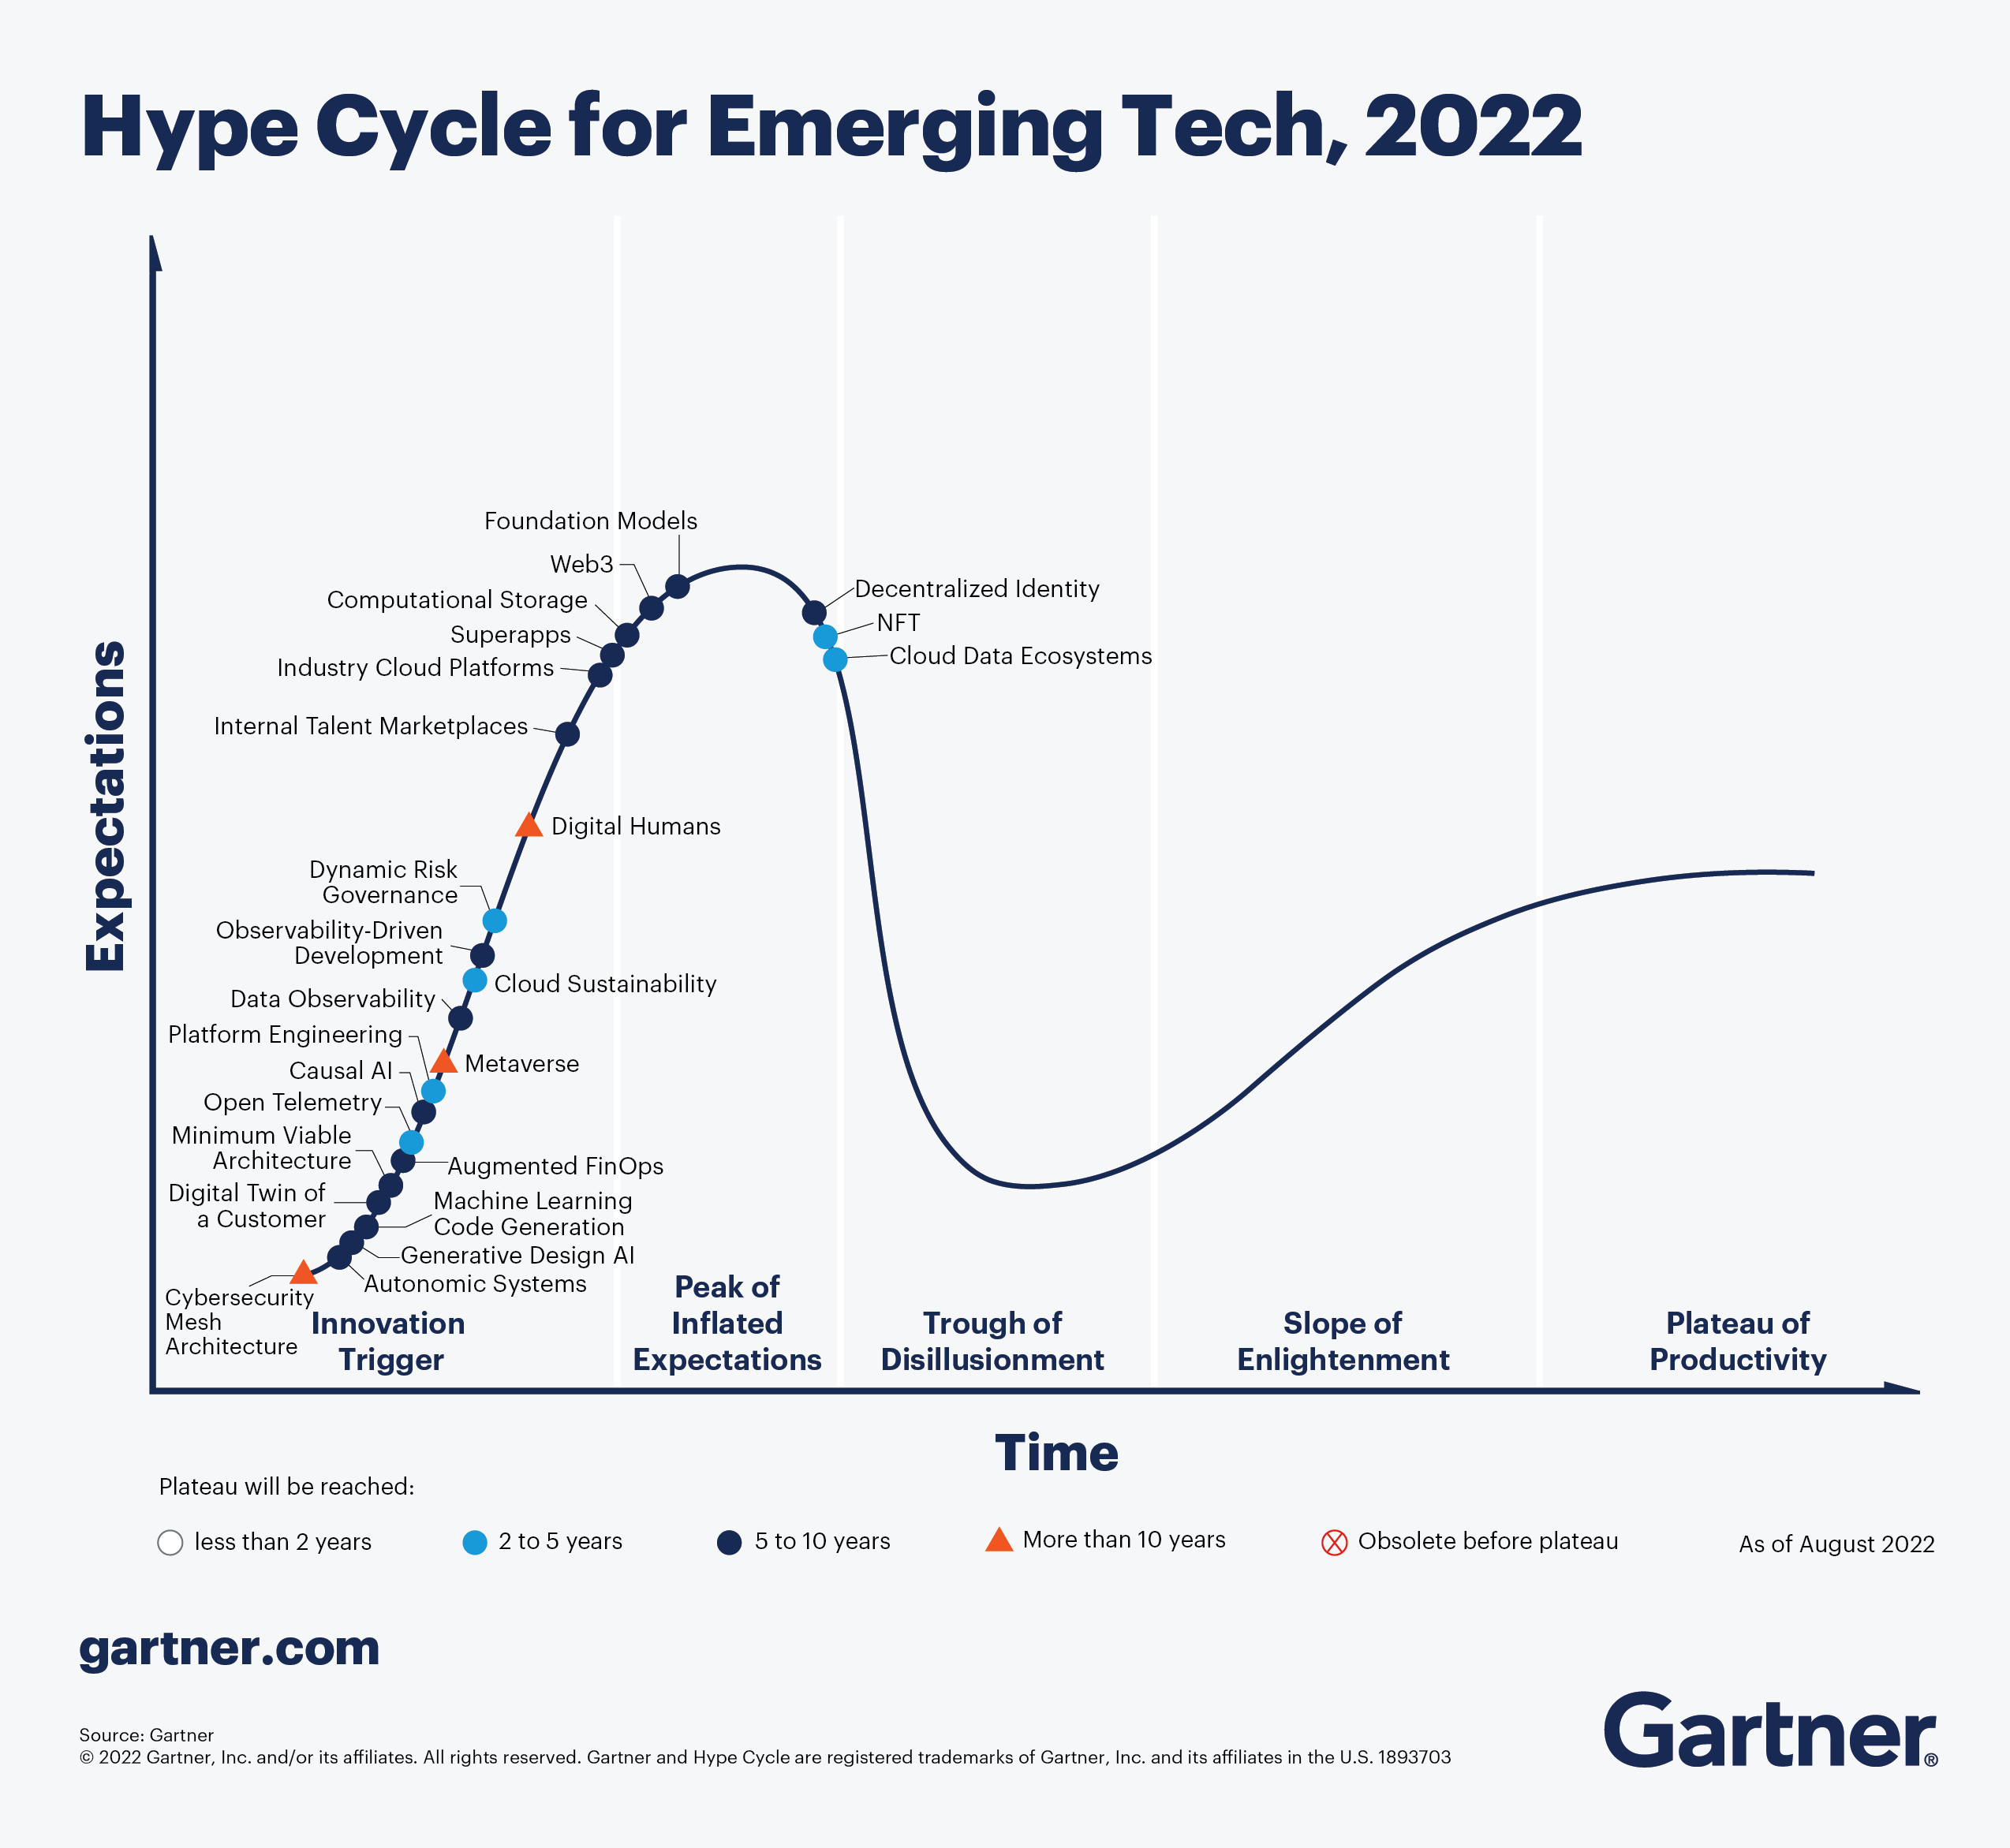
\includegraphics[width=0.9\linewidth]{gartners}
	\caption{The Gartners Hype Cycle for 2022.}
	\label{fig:gartners}
\end{figure}
With all this attention it seems timely to explore the potential of recent technologies, which can address metaverse interactions in \textit{business to business} (B2B), \textit{business to customer} (B2C), and the newer C2C (social commerce; \textit{creator to consumer, customer to customer, consumer to consumer\cite{jones2008trust})}. \par %Figure \ref{fig:landscapevenn} demonstrates how some of these domains intersect.\par
This book seeks to overview and explain the available open source technologies. It supports an open source \href{https://github.com/flossverse/product}{github repository} which enables SMEs to access these emergent platforms and ecosystems. It aims to build toward a minimum viable product for trust minimised transfer of value within a social immersive space, but also across all internet connected devices.\par
Referencing is in two styles; academic works and books are numeric, while opinion pieces, gray statistics, and pertinent news articles are hyperlinked from the text. This hybrid style yields about twice the citation density of a normal PhD thesis, which is a lot. For this reason the normal blue hyperlink colour was eschewed in favour of a more aesthetic ``gray''. \par%There is also a version of the PDF which complies with accessibility best practice if this is a problem.  \par 
%\subsection{Notes on progress}
%\textbf{This version of the book is being overhauled to improve the focus, and expand the virtual production use cases. It may be inconsistent and look scrappy until this message is removed.}
